\documentclass[twoside]{article}

\newenvironment{Figure}
  {\par\medskip\noindent\minipage{\linewidth}}
  {\endminipage\par\medskip}

\newcommand{\repo}{Our code repository can be found here: \url{http://code.google.com/p/590networks/}}
\newcommand{\amznSrc}{Haselgrove, H. "Using the Wikipedia page-to-page link database." Retrieved from \url{http://haselgrove.id.au/wikipedia.htm}.}
\newcommand{\wikiSrc}{J. Leskovec, L. Adamic and B. Adamic. (2007). "The Dynamics of Viral Marketing." $ACM Transactions on the Web (ACM TWEB)$. 1(1). Retrieved from \url{http://snap.stanford.edu/data/amazon-meta.html}}
\newcommand{\jgraphtSrc}{JGraphT website: \url{http://jgrapht.org/}}
\newcommand{\labsSrc}{\url{http://google.about.com/od/blogs/ss/Google-Labs-Dropouts-And-Failures.htm}}

% ------
% For pretty math
\usepackage{amsmath}

% ------
% Images
\usepackage{graphicx}

% ------
% Fonts and typesetting settings
\usepackage[sc]{mathpazo}
\usepackage[T1]{fontenc}
\linespread{1.05} % Palatino needs more space between lines
\usepackage{microtype}


% ------
% Page layout
\usepackage[hmarginratio=1:1,top=32mm,columnsep=20pt]{geometry}
\usepackage[font=it]{caption}
\usepackage{paralist}
\usepackage{multicol}

% ------
% Lettrines
\usepackage{lettrine}


% ------
% Abstract
\usepackage{abstract}
	\renewcommand{\abstractnamefont}{\normalfont\bfseries}
	\renewcommand{\abstracttextfont}{\normalfont\small\itshape}


% ------
% Titling (section/subsection)
\usepackage{titlesec}
\renewcommand\thesection{\Roman{section}}
\titleformat{\section}[block]{\large\scshape\centering}{\thesection.}{1em}{}


% ------
% Header/footer
\usepackage{fancyhdr}
	\pagestyle{fancy}
	\fancyhead{}
	\fancyfoot{}
	\fancyhead[C]{CS590 Final Paper $\bullet$ April 2013 }
	\fancyfoot[RO,LE]{\thepage}


% ------
% Clickable URLs (optional)
\usepackage{hyperref}

% ------
% Maketitle metadata
\title{\vspace{-15mm}%
	\fontsize{24pt}{10pt}\selectfont
	\textbf{Analyzing the Semantic Modeling Capabilities of Google Sets}
	}	
\author{%
	\large
	\textsc{Azfar Khandoker}\\
	\normalsize	Purdue University \\
	\normalsize	\href{mailto:akhandok@purdue.edu}{akhandok@purdue.edu}
    \and
    \textsc{Ryan Miller}\\
	\normalsize	Purdue University \\
	\normalsize	\href{mailto:millerrv@purdue.edu}{millerrv@purdue.edu}
	\vspace{-5mm}
	}
\date{}



%%%%%%%%%%%%%%%%%%%%%%%%
\begin{document}

\maketitle
\thispagestyle{fancy}

\begin{abstract}
\noindent
In this paper we abstract data retrieved from Google Sets and transform the semantic 
concepts into a graph representation that we can further analyze. We use this representation to 
determine the potential of using Google Sets as a network building tool. We compare the generated 
graph with the graph representations of other online services, including Amazon co-purchasing and 
Wikipedia entries. We look for small world characteristics in all three networks. Finally, we show 
the similarities between these semantic networks using cosine similarity, and investigate the 
potential of using Google Sets as a product recommendation engine.
\end{abstract}

\begin{multicols}{2}
\section{Introduction}
There are many semantic networks publicly available. Amazon's co-purchasing dataset, which shows the
 products that are purchased together on amazon.com, and Wikipedia are a couple of the more 
 interesting ones we examine in this paper. Google Sets, a public service provided by Google, 
 associates a word or a list of words with a set of other words or lists of words, thus providing 
 semantically similar results for a given query. All three of these services and their interactions 
 therein can be abstracted into a graph representation, where semantic words or phrases make up the 
 nodes in each network. In this paper, we describe how we transformed data retrieved from Google 
 Sets into a graph that represents it as a semantic network. We also rigorously compare this network
 against the Amazon co-purchasing data set and the Wikipedia data set. We explore the possible 
 implications of the similarities and the differences between these networks. 
 
 \subsection{Semantic Networks}
 Popular in the fields of linguistics, psychology, and artificial intelligence, semantic networks 
 are graphs used to illustrate the interconnectedness behind  knowledge \cite{shapiro92}. Although 
 semantic networks can be structured to provide relationships (for example, hierarchy and 
 inheritance), they can also model related concepts by connecting similar words or concepts with an 
 edge. Our project explores characteristics behind semantic networks, such as the small world 
 phenomenon and cosine similarity. In addition to established semantic networks, such as the 
 Wikipedia online encyclopedia, we  have implemented a strategy to build networks using data 
 provided from Google Sets. 
 \begin{Figure}
 \centering
 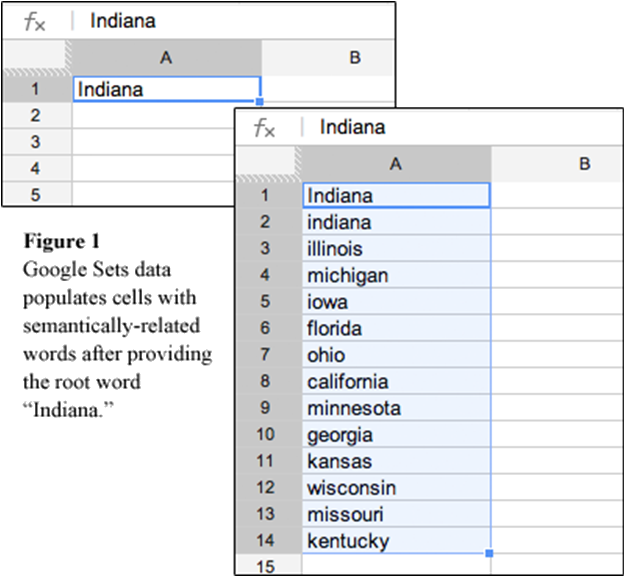
\includegraphics[width=\columnwidth]{pic1.png}
 \end{Figure}
 
 \subsection{Google Sets and Comparison Networks}
 Originally designed to add semantic language capability to search queries, Google Sets is a former 
 Google Labs project released to the public in 2002\footnote{\labsSrc}. Despite being discontinued in 
 2011, data from Google Sets is still available through Google's cloud-based spreadsheet application
 . After entering a word into a spreadsheet cell, the user can hold the 'CTRL' or 'ALT' key and drag
 the bottom-right corner to cause semantically-related words to appear in the cells below the source
 word (Figure 1).
 \begin{table*}[ht]
 \caption{Comparison semantic networks}
 \centering
 \begin{tabular}{p{0.25\linewidth}p{0.25\linewidth}p{0.25\linewidth}}
  & Wikipedia Snapshot & Amazon Co-purchasing\\
 \hline
 Number of nodes & 5.7 million & 542,000\\
 Number of edges & 130 million & 1.2 million\\
 Average degree & 45.531 & 4.538\\
 Average path length & Unavailable & 2.842\\
 Global Clustering Coefficient & 0.014 & 0.215\\
 \end{tabular}
 \label{tab:semanticNetworkComparison}
 \end{table*}
 
 Google Sets provides a wealth of data derived from real-world searches that we aimed to utilize in 
 our project, but we required a baseline to make sense of the semantic networks generated by Google 
 Sets. Specifically, we compared networks created from Google Sets to other semantic networks, 
 including the links among Wikipedia articles and product co-purchasing data from Amazon shopping 
 (Table \ref{tab:semanticNetworkComparison})\footnote{\amznSrc}\textsuperscript{,}\footnote{\wikiSrc}. In the 
 Wikipedia network, directed edges indicate that an article (encyclopedia entry) links directly to 
 another article. Wikipedia editors can insert links arbitrarily into articles, leading to a well-
 connected network in which a Wikipedia article, on average, links to 45 other articles. In the 
 Amazon co-purchasing network, nodes are represented by products (books, films, andothers) available
 for sale on the Amazon website.  When an Amazon user purchases multiple items simultaneously, edges
 are added to the network to reflect "co-purchasing" conditions. Thus, according to our Amazon data 
 set, an Amazon user, on average, purchases around 4 items together.

\section{Problem Definition}
First, we investigate whether the Google Sets data exhibits a small world phenomenon, especially in 
comparison to Wikipedia and Amazon co-purchasing networks. We then highlight the overlap between 
data from Google Sets and Amazon co-purchasing and determine whether the data can thus be used as a 
refinement tool for product recommendation engines. Google Sets, stemming from users' search queries
, may therefore offer an ideal secondary source for recommendations. Finally, we address the issue 
of selecting the best candidate words from the network to recommend using the concept of cosine 
similarity, expanding on a study looking at semantic similarity of words and their synonyms appearing in 
the Roget's Thesaurus \cite{steyvers01}.

 \subsection{Related Work}
 Milgram was one of the first researchers to explore small world characteristics of a graph, noting 
 the surprisingly short path lengths required to reach two non-neighbor individuals in a societal 
 network \cite{milgram67}. He found a median of five hops required for two individuals to communicate 
 (corresponding to an average path length of five, a bound we later observe in Google Sets data). 
 Semantic networks in particular have also been shown to exhibit small world characteristics, such 
 as English words and their synonyms, studied by \cite{steyvers01}.
 
 Networks have also been used to generate recommendations, such as the use of membership statistics 
 in social networks to predict movie recommendations \cite{golbek06}.  Semantic networks can also 
 aid in producing recommendations, such as a system that recommends music based on the semantic 
 similarities of genres placed in a network \cite{crossen02}.
 
 \subsection{Models, Measures and Algorithms}
 We use the metrics of average path length and degree distribution as described by Barab�si and 
 Albert \cite{barabasi02} and clustering coefficient as described by Watts and Strogatz \cite{watts98} to show whether 
 a network is a small world network or not. As an important analysis tool used to further 
 distinguish small world networks, we look for a power law degree distribution (Equation 
 \ref{eq:powerLaw}), rather than an exponential degree distribution, which does not indicate the 
 same types of hubs present in small world networks.
 
 \begin{equation}
 p(x) \propto x^{-\alpha}
 \label{eq:powerLaw}
 \end{equation}
 
 In addition to small world characteristic, we explore overlap of the networks with each other by 
 comparing the results given by a traversal of each graph and counting the identical nodes 
 encountered \cite{lauder98}. Finally, we use the notion of cosine similarity to show 
 the similarity of the networks on a deeper semantic level compared with examining average path 
 length and degree distribution \cite{salton75}. Under the cosine similarity model (Equation 
 \ref{eq:cosSim}), rows in the network's adjacency matrix for two nodes are represented as vectors. 
 When two nodes share many of the same neighbors, their cosine similarity score will be higher, 
 indicating higher similarity between these two terms in semantic networks. As a product 
 recommendation engine, these similar semantic terms will make ideal candidates for recommendation.
 
 \begin{subequations}
  \begin{equation}
  \sigma_{ij} = \cos{\theta} = \frac{n_{ij}}{\sqrt{d_id_j}}
  \end{equation}
  \begin{equation}
  n_{ij} = \displaystyle\sum\limits_{k}A_{ik}A_{kj}
  \end{equation}
  \label{eq:cosSim}
 \end{subequations}

\section{Implementation}
Our implementation consists of a Java application that we used to generate a graph representation of
 Google Sets. We also used various Python scripts to generate graphs of the Wikipedia dataset as 
 well as the Amazon co-purchasing dataset. We also used Python scripts to run various analyses on 
 the graphs.\footnote{\repo}
 
 \subsection{Google Sets Network Builder}
 Google Sets was only accessible via the Google Spreadsheet ("the spreadsheet") that is available as
 a part of Google Drive at the time of our studies. As such, a user would have to manually invoke 
 the service by following the procedure we mentioned earlier. We needed to automate this process to 
 allow for continued data retrieval even in the absence of human interaction. We created a robot to 
 perform the user's actions using the Java libraries. We invoked the robot to perform these and 
 other actions when we needed actions to be performed by the user. We also interfaced with the 
 spreadsheet API to retrieve the results from Google Sets as well as fill in the spreadsheet with 
 new data to be used with Google Sets. Finally, we used the $JGraphT$\footnote{\jgraphtSrc} library 
 to generate our graph.
 \begin{Figure}
 \centering
 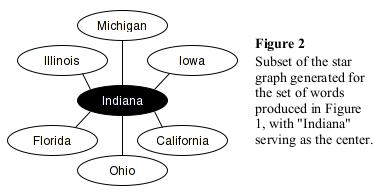
\includegraphics[width=\columnwidth]{pic2.png}
 \end{Figure}
 \setcounter{figure}{2}
 
 Every time we used Google Sets through the spreadsheet, we started with a seed word, $s$. For a 
 seed word, we received a result set from Google Sets, $R = \{ r_1 , r_2 , \ldots , r_n \}$, of $n$ 
 result words where $r_i$ denotes the $i$th result word. For every result word, we first checked if 
 the result word matched a predefined regular expression. We did this to filter out any invalid 
 words that we did not want to consider (e.g. words not in the English language or words containing 
 numbers or symbols). The initial results for a seed word generate a star graph with the seed word 
 as the central node (Figure 2).
 
 \subsection{Not Just a Collection of Stars}
 Next, we checked to see if $r_i$ was the same as $s$ for any $i$. If so, we ignored this result 
 because we did not allow for self-loops in the graph. Finally, if the $i$th result was not already 
 present in the graph, we created a node to represent it. If the result is already present in the 
 graph, we did not create a new node for it, instead creating an edge between the node that 
 represented $r_i$ and the node that represented $s$ and added it to the graph. Anytime we added a 
 result word to the graph, we also added it to a queue of words that would give us the next $s$. We 
 would repeat this procedure for all results in $R$.
 
 One can think of Google Sets returning a star graph for each $s$. $s$ would be the central node 
 with each word in the returned $R$ being the neighbors of it. However, since we only created a node
 for a word in $R$ if and only if it was not already present in the graph, the structure of a star 
 graph quickly dissipates since we would create edges between pre-existing nodes in the graph. For 
 example, the result set may be $R_{Indiana} = \{$ "Michigan" , "Iowa" , "Illinois" $\}$ for $s$ = 
 "Indiana". This is a star graph. However, on the next iteration when we use $s$ = "Michigan", we 
 may get a result set $R_{Michigan} = \{$ "Illinois" , "Minnesota" , "Indiana" $\}$. We see that our
 graph is no longer a set of star graphs, since we have a triangle consisting of the nodes $\{$ 
 "Indiana" , "Michigan" , "Illinois" $\}$.
 
 \subsection{Analysis Tools}
 To analyze the graphs of Google Sets, Wikipedia and Amazon co-purchasing, we used the $igraph$ 
 library along with our own implementations of some analysis metrics. We relied on the standard 
 $igraph$ implementations of \texttt{degree\_distribution()} and \texttt{path\_length\_hist()} when 
 looking for small world characteristics. For the Wikipedia data set, at over 6 gigabytes in GML 
 format, $igraph$ was unable to return an average path length. Instead, we looked at various 
 subgraphs to analyze this network property. When generating subgraphs at depth $k$ from a source 
 node, we rely on the \texttt{neighborhood()} procedure in $igraph$, which provides a useful way to 
 examine subgraphs in large networks.
 
 The $igraph$ tool has no built-in procedure for cosine similarity, so we implemented this analysis 
 technique in Python based on the formula provided in class (Equation \ref{eq:cosSim}). We also relied 
 on standard graphing tools, such as Python's \texttt{matplotlib} and $Microsoft\ Excel$ to analyze 
 properties of the degree distribution curves and power law regression values.
 
\section{Studies}
 We conducted various studies on the graphs to see how the data contained in them may be similar and 
 semantically related. We studied the small world characteristics of each of the networks and we also
 analyzed their semantic similarities.
 
 \subsection{Small World Characteristics}
 To show the presence of small world phenomena, we analyzed the graphs using various metrics 
 including average path length, clustering coefficient and degree distribution. When we analyzed the
 graphs, we ran a simple experiment on all three graphs to see how they each performed using the 
 same input. We ran our algorithm with an initial seed of $s$ = "wine". We ran our algorithm until 
 we either reached a depth of $k$ = 4 or we found that one of the words in a returned $R$ was the 
 word "france". We summarize these findings in Table \ref{tab:wineFrance}. This generated a subgraph
 for each of the three graphs. We used these subgraphs in our analyses. We summarize these subgraphs
 in Table \ref{tab:subgraphs}. For the average path length and the clustering coefficient, we have 
 also included some other data. The data in the parenthesis are the corresponding values for an 
 Erdos-Renyi random graph \cite{erdos59} ("the random graph") with the same number of nodes 
 and edges as the graph with which it is being compared (i.e. for the Google Sets subgraph, we 
 created an Erdos-Renyi random graph with 2,871 nodes and 8,962 edges).
 \begin{table*}[ht]
 \caption{Shortest paths from "wine" to "france"}
 \centering
 \begin{tabular}{| p{0.25\linewidth} | p{0.25\linewidth} | p{0.25\linewidth} |}
 \hline
 Network & Path Length & Path\\
 \hline
 Google Sets & 4 & "wine" $\rightarrow$ "champagne" $\rightarrow$ "bordeaux" $\rightarrow$ "france"\\
 \hline
 Wiki & 1 & "Wine" $\rightarrow$ "France"\\
 \hline
 Amazon & 4 & "Wine" $\rightarrow$ "Italy (Culinaria)" $\rightarrow$ "Culinaria: The United States: A Culinary Discovery (Culinaria)" $\rightarrow$ "Culinaria France (Culinaria Series)"\\
 \hline
 \end{tabular}
 \label{tab:wineFrance}
 \end{table*}
 \begin{table*}[ht]
 \caption{Small world characteristics in comparison networks}
 \centering
 \begin{tabular}{p{0.2\linewidth}p{0.2\linewidth}p{0.2\linewidth}p{0.2\linewidth}}
 & Google Sets & Wikipedia & Amazon\\
 \hline
 \# nodes & 2,871 & 544 & 1,373\\
 \# edges & 8,962 & 25,403 & 3,432\\
 Avg. degree & 6.243 & 93.393 & 5.998\\
 \textbf{Avg. path length} & \textbf{4.329 (4.554)} & \textbf{2.344 (1.828)} & \textbf{4.287 (4.640)}\\
 \textbf{Clustering coeff.} & \textbf{0.255 (0.002)} & \textbf{0.727 (0.172)} & \textbf{0.343 (0.003)}\\
 \end{tabular}
 \label{tab:subgraphs}
 \end{table*}
 
 For average path length, only the Wikipedia data set demonstrated a higher average path length than
 that of the random graph; the other two graphs show a smaller average path length. This uniqueness 
 of Wikipedia among the other subgraphs is also apparent for the clustering coefficient. The 
 clustering coefficients of Google Sets and Amazon are 128\% and 114\% higher than the random graph 
 that coincides with them, respectively. However, for the Wikipedia data set, the clustering 
 coefficient is merely 4\% higher than that of the random graph for 
 Wikipedia. Using these values, we can see that both Google Sets and Amazon demonstrate small world 
 phenomenon characteristics but Wikipedia does not. Small average path length and large clustering 
 coefficient (compared to random graphs of equal density) are necessary, but not sufficient 
 conditions for a graph to be considered small world. We examined another characteristic, degree 
 distribution, of the three graphs to further emphasize the presence, or absence, of small world 
 phenomena in these graphs.
 
 Figures \ref{fig:googleSets}, \ref{fig:wiki} and \ref{fig:amzn} show the degree distributions of 
 the three subgraphs of Google Sets, Wikipedia and Amazon, respectively. We have also included the 
 power trendline equation for each of the graphs. We see that the equations for the Google Sets and 
 Amazon subgraph demonstrate a power law degree distribution. For Equation \ref{eq:powerLaw} to be 
 valid for a power law degree distribution, we expect an exponent value $2 < \alpha < 3$ 
 \cite{clauset09}. Contrary to this, the Wikipedia data set does not have an $\alpha$ value 
 within this range. We also see that the $R^2$ value for both Google Sets and Amazon are much higher
 than that for Wikipedia, indicating a strong power function curve fit. Such results are evident 
 from examining the plots visually, as well. On a log-log scale, a power law degree distribution 
 should resemble a line, which is shown by both Google Sets and Amazon. Wikipedia does not show the 
 same behavior on a log-log scale plot. Thus it follows that a power law trend line was not a good 
 fit for the degree distribution in the Wikipedia data set. We therefore conclude that the Wikipedia
 data set does not contain a power law degree distribution contrary to Google Sets and Amazon.
 \begin{Figure}
 \centering
 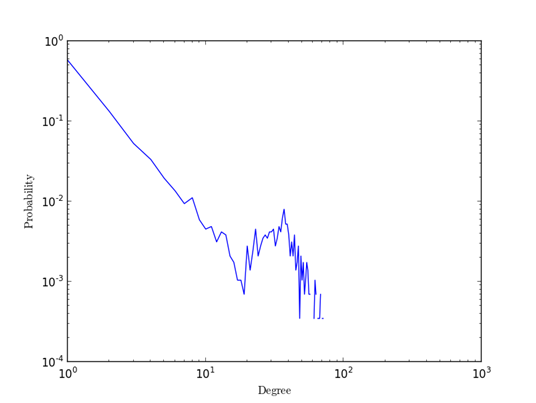
\includegraphics[width=\columnwidth]{pic3.png}
 \captionof{figure}{Google Sets - $p(x) = 0.174x^{-1.293}$ , $R^2 = 0.724$}
 \label{fig:googleSets}
 \end{Figure} 
 \begin{Figure}
 \centering
 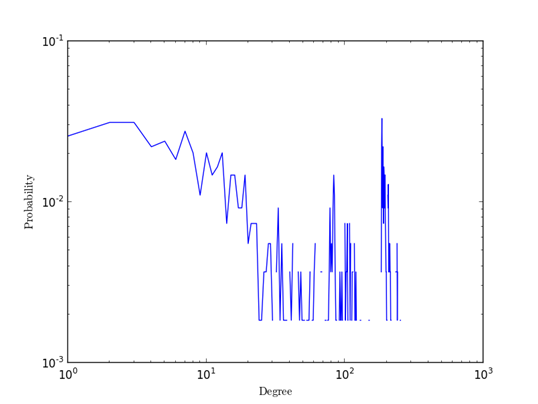
\includegraphics[width=\columnwidth]{pic4.png}
 \captionof{figure}{Wikipedia - $p(x) = 0.018x^{-0.341}$ , $R^2 = 0.197$}
 \label{fig:wiki}
 \end{Figure} 
 \begin{Figure}
 \centering
 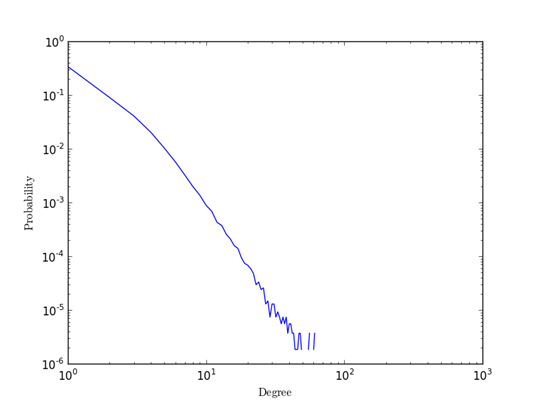
\includegraphics[width=\columnwidth]{pic5.png}
 \captionof{figure}{Amazon - $p(x) = 0.878x^{-3.172}$ , $R^2 = 0.964$}
 \label{fig:amzn}
 \end{Figure}
 
 \subsection{Comparison of Semantic Networks}
 Comparing degree distribution and average path length give a global view of the entire network, but
 we also explore the actual words present in the network to see how the networks overlap, i.e. 
 contain the same set of words. When we compare the nodes present in the Google Sets network for a 
 seed word of "Oreo", we find high overlap with nodes present in the Amazon network, while this 
 overlap is absent in comparison with the Wikipedia network (Tables \ref{tab:oreoSem} and 
 \ref{tab:matching}).
 \begin{table*}[ht]
 \caption{Semantic networks generated with a seed word of "Oreo"}
 \centering
 \begin{tabular}{p{0.2\linewidth}p{0.2\linewidth}p{0.2\linewidth}p{0.2\linewidth}}
 & Google Sets & Wikipedia & Amazon\\
 \hline
 \# nodes & 10,229 & 16,478 & 1,119\\
 \# edges & 33,081 & 1,252,227 & 1,118\\
 \end{tabular}
 \label{tab:oreoSem}
 \end{table*}
 \begin{table*}[ht]
 \caption{Node matching among the semantic networks}
 \centering
 \begin{tabular}{p{0.15\linewidth}p{0.15\linewidth}p{0.15\linewidth}p{0.15\linewidth}p{0.15\linewidth}}
 & Unique for Google Sets & Not in Google Sets & Shared & Percentage Shared\\
 \hline
 Google Sets vs. Wiki & 9,682 & 15,931 & 547 & 3.320\%\\
 Google Sets vs. Amazon & 9,919 & 809 & 310 & 27.703\%\\
 \end{tabular}
 \label{tab:matching}
 \end{table*}
 
 Such a high overlap between Google Sets and Amazon data sets may imply a potential use for data 
 generated from Google Sets as a product recommendation engine. While Amazon currently recommends 
 products based on products purchased together (co-purchasing data), Google Sets can supplement 
 recommendations by returning related words and phrases that users have searched for on Google. When
 these semantic concepts correspond to products listed on Amazon (for instance, when a word or set 
 of words appears in the item's title), this product can then serve as a candidate recommendation 
 for an Amazon user.
 
 \subsection{Using Semantic Similarity for Further Refinement}
 Finding related words with short path lengths in the Google Sets network may return many 
 suggestions, but a short path length alone does not guarantee that such suggestions are relevant. 
 For example, in the "wine" to "France" graph we generated, "drink" appears immediately connected to
 "wine" (with a path length of 1). But despite the close proximity in the graph, users interested in
 products stemming from "wine" are likely not interested in every beverage available on Amazon.  To 
 prune and refine these suggestions, we can use the concept of cosine similarity, which relates 
 semantically similar concepts by quantifying the number of shared neighbors of each of the nodes 
 (Salton, 1975).
 
  \begin{table*}[ht]
 \caption{Cosine similarity scores between "wine" and related terms in each network studied}
 \centering
 \begin{tabular}{p{0.2\linewidth}p{0.2\linewidth}p{0.2\linewidth}p{0.2\linewidth}}
 & Google Sets & Wikipedia & Amazon\\
 \hline
 wine $\rightarrow$ france & 0.0 & 0.0058 & 0.0096\\
 wine $\rightarrow$ grape & 0.0 & 0.02229 & 0.0344\\
 wine $\rightarrow$ alcohol & 0.1427 & 0.00921 & 0.0094\\
 wine $\rightarrow$ beer & 0.8007 & 0.1987 & 0.6862\\
 \end{tabular}
 \label{tab:cosSim}
 \end{table*}
 
 When we examine cosine similarity scores for "wine" and related terms in the "wine" to "france" 
 graphs generated from each network we studied (Table \ref{tab:cosSim}), we can further refine our 
 product recommendations. From the similarity scores, it becomes clear that although "grape" may 
 appear in the network connected to "wine", these terms are not necessarily similar.  By computing 
 cosine similarity between "wine" and every other term in the network, we can identify the most 
 similar words, such as "beer". Therefore from our original product recommendations, we can prune 
 many terms while maintaining such similar terms as "beer".
 
\section{Results}
Here we discuss our findings and the implications they have on the interrelationships of the data 
 sets we have examined in this paper. First, we discuss what the meaning of a shortest path 
 indicates in the networks we studied and how networks generated from Google Sets exhibit this 
 behavior. Next, we comment on the overlap between the three semantic networks, noting a higher 
 overlap between Google Sets and Amazon networks than Google Sets and Wikipedia. Finally, we 
 re-define cosine similarity and note its ability to find similarity between nodes on a deeper level
 than network analysis alone.
 
 \subsection{Discussion}
 In our previous work, we showed the shortest path characteristics of the data sets that 
 we examined throughout this paper. By running our implementation, we retrieved a path from "wine" 
 to "france" using Google Sets. This information can be used as a supplement to a recommendation 
 engine due to its linking of semantic concepts from a seed word to a target word.
 
 Recommendations cannot be arbitrarily applied to any network, however. The network we choose to 
 compare to Google Sets should share many of the same nodes, implying an overlap of the semantic 
 structure of the network. Amazon currently has a recommendation engine that bases its 
 recommendations on the co-purchasing data a customer has. As shown in Table \ref{tab:matching}, 
 networks generated from Google Sets and Amazon overlap to a high degree. If Amazon were to use 
 Google Sets as well, then the combination of the co-purchasing data along with the data available 
 in Google Sets would allow Amazon to make more meaningful recommendations that are not based solely
 on co-purchasing data for that customer.
 
 As we have seen, high network overlap and short path lengths do not always represent ideal 
 recommendation candidates, however. To further prune the set of recommendations, we can employ 
 semantic similarity in the form of cosine similarity, which relates nodes that share common 
 neighbors in a network. Using cosine similarity, we can then make strong product recommendations 
 based on data from the network generated from Google Sets.
 
 \subsection{Future Work}
 The techniques and algorithms and analyses we discussed in this paper can be arbitrarily expanded 
 to any number of graphs. For example it may be interesting to study how the results in Google Sets 
 follow the co-purchasing data of Amazon along with status updates that are made on social networks 
 like Facebook and Twitter. These can also be linked to recent events in the news by examining 
 graphical representations of recent articles from $The\ New\ York\ Times$.
 
 It may also be possible to see how Google Sets can be applied to the discipline of psychology. 
 The human mind can retrieve words similar to a result set like we described when given an initial 
 word like a seed word. Further studies can be done to see how the results returned by Google Sets 
 can be used to model the human brain and speech pathology of the human psyche.
 
 \section{Conclusion}
 In this paper we have examined the Google Sets semantic relationship service available from Google 
 via the Google Spreadsheet interface. We have designed and implemented a tool that will generate a 
 graphical representation of the data available in Google Sets. We can then compare this graphical 
 representation to graphical representations of two other data sets (Wikipedia and Amazon 
 co-purchasing data) and run analyses to discover various characteristics common to the semantic 
 networks. We examined which networks demonstrate small world behavior by examining their average
 path lengths, clustering coefficients and their power law degree distributions. The small world 
 characteristic present in Google Sets allows us to relate concepts with short path lengths, and 
 thus hints at the ability to recommend semantically-related concepts. Due to the high overlap in 
 shared nodes between Google Sets and Amazon networks, we determined that Google Sets may be able to
 improve product recommendations typically made through Amazon co-purchasing data. Finally, we 
 examined how semantic similarity can finalize these recommendations by narrowing the set to words 
 and phrases that have been deemed semantically-similar, sharing many of the same neighbors in the 
 same network.
 
 \bibliographystyle{unsrt}
 \bibliography{report}
\end{multicols}
\end{document}
